\chapter{Introduction}
Enormous datasets are a common case in today's applications. Compressing these datasets is often beneficial, because doing so 
naturally decreases memory requirements, but also can make it faster to transfer data from disk to memory \citep{Zob95}. 

Fundamental method for data compression is variable-length coding \citep{Sal99}. The main idea of variable-length encoding is that 
frequent sequences of data are represented with shorter codewords. Because the sequences of data have different lengths when compressed, it is 
not trivial to determine the exact location of a certain element in the compressed data. If this is required, the usual 
data compression algorithms are inefficient. Fortunately, such random access to elements is not a requirement compression algorithms usually 
need to fulfill. 

However, random access to compressed data is very useful in compressed data structures. It saves storage space, bandwidth and 
increases the likelihood of data already being in cache \citep{Sch02}. In most compression methods, the only way to do this is to decompress data 
from the beginning. 

Variable-byte encoding is a method for compressing integers of different byte length. An additional \textit{continuation bit} is added to the data to denote whether the compressed integer
is continued to the next byte or not. Two different light-weight data structures are built over the continuation bit array. $Rank_1$($i$) returns the number of 1 bits in the bit array between 
indexes 0 and $i$-1. $Select_1$($i$) returns the index of the i-th 1 bit in the array. The fact that the compressed data blocks are of the same size is used
with the data structures to allow direct access to the compressed variable-byte data.

A variable-byte encoding based integer compression method with fast random access was first introduced by \citep{Bri09}. They used a clever block 
reorganizing and a $rank$ data structure to achieve random access. Their solution is currently the only published solution for the problem and it 
has been widely adopted \citep[e.g.][]{Kon17, Sha16}. 

In this thesis, an alternative solution that instead makes use of a $select$ data structure is proposed and explained in detail. Comparison to the $rank$-based 
implementation by Brisaboa et al is provided with different implementations of $rank$ and $select$ and several different data sets. The proposed method does not use data 
reorganizing, but rather capitalizes on the assumption that data is encoded the same way it is in the source. Because variable-byte encoding does not assign 
new codewords to data when encoding, data can be read straight from the memory and reassembling the integer from blocks is not needed.

Because of the block reorganizing, the $rank$ does not infact need a $rank$ query when fetching small elements. This makes the $rank$ method superior when dataset contains 
mostly small integers. With larger integers, the decoding needs multiple $rank$ calls and the new $select$-based method performs better. 

Decompressing a subarray is experimented later in this thesis. Due to how the data is stored, the proposed $select$ method offers fast access to the next or previous element. This makes a 
subarray decompression very convenient and fast. Solutions for subarray fetching with both $rank$ and $select$ methods are proposed and compared. $Select$ based method performs better due to its 
single $select$ call requirement, while the $rank$ call amount depends on the size of the largest element in the subarray.

\chapter{Variable-byte encoding of integers}

Variable-byte (VB) encoding \citep{Wil99} is a method for compressing unsigned integers via omitting leading zero bits that would be present in a longer fixed 
width word. In normal data sets, VB encoding loses in compression performance to generic algorithms like Huffman encoding or Lempel-Ziv encoding, but 
is generally faster to decode \citep{Bri09} and so is sometimes preferred, also  due to its simplicity of implementation.

A good data set for VB encoding is a list of mostly small integers with a need to support larger ones. A search engine may use an inverted index of 
words in documents. For each word, a list of document IDs where the word appears is stored. It may also store locations of the word in document for 
advanced search purposes. Usually these lists are preprocessed to an inverted index, storing each number as its difference to the previous number 
instead of the actual number \citep{Man08}. Common words have a lot of entries in these lists, but inverted index encoding makes the integers are small. 
In contrast, rare words have only a few entries but the integers stored are larger. These lists are thus excellent candidates for VB encoding. 

Variable-byte encoding originates from and is used in the MIDI music file format \citep{Mid96} and several applications have a similar implementation of VB. Apache 
Lucene has the vInt datatype \citep{ApaLV} which works well with short inverted index lists \citep{Wan09}. The Wireless Application Protocol has a variable length unsigned integer uintvar, Google Protocol Buffers has a Base 128 Varint \citep{GooPB},
 Microsoft .Net framework offers "7BitEncodedInt" in BinaryReader and BinaryWriter classes and IBM DB2 uses variable byte encoding to store record identifier lists \citep{Bha09}.

Later, VB encoding was found to be efficient for compressing integer lists. It was first experimented as a tool for compressing inverted index lists of word locations in documents by \citep{Sch02}. 
In that setting, VB codes yielded excellent results, and since then many different approaches have been introduced. 

More recent studies have taken a look into the machine code level for VB and applied SIMD (Single instruction, multiple data) instructions for VB decoding \citep{Lem18,Pla15}. The bit 
operations in VB are simple and therefore modifying the code to use SIMD instructions is straightforward and the speed improvements are significant. 

Elias Delta and Gamma codes \citep{Eli75} are popular encoding methods for the aforementioned data sets. Their encoding process assigns short bit sequences to small integers, 
which is why they outperform in terms of compression VB encoding on datasets containing a lot of small integers \citep{Wil99}, such as inverted indexes \citep{Anh05, Pib19}. In this thesis, 
the data sets used for experimentation will have the focus on slightly larger, unordered numbers.

\section{VB encoding}
The name \textit{variable-byte} is reflected in how the integers are stored. When stored in an array, each element requires the same amount of space. This is very inefficient if a lot of the values are 
very small but the array also has to support very large integers. VB encoding attempts to eliminate the unneeded leading zeros. The bits in an integer are split into blocks of length $b$ and empty blocks 
from the beginning are discarded. Because the lengths of the integers may now be different, the data cannot be stored as it is. Instead a \textit{continuation bit} is added in front of each block to form 
a $chunk$. This bit is set to 0 on all chunks except for the last one which contains the least significant bits. The continuation bit is used in decoding to signal whether or not the current integer 
continues in the next chunk.

For example, the standard 16-bit representation of an unsigned integer 42 is \texttt{00000000 00101010}. Assuming the block length is 4, it is split to \texttt{0000 0000 0010 1010}. The empty blocks 
are removed from the beginning and then the continuation bits are added. 1 is added in front of the last block (containing the least significant bits) and 0 to the other blocks, resulting in 
\texttt{\underline{0}0010 \underline{1}1010}. Table~\ref{table:vbytes} contains examples of VB encoded integers with byte length 4. 

\begin{table}
\centering
\begin{tabular}{l||c c c c c} 
Original number & first block & second block & third block & fourth block &\\ 
\hline \hline 
4  & \texttt{\underline{1}0100}    &                             &                           &  &  \\
17  & \texttt{\underline{0}0001}   & \texttt{\underline{1}0001}  &                           &  &  \\
620  & \texttt{\underline{0}1100}  & \texttt{\underline{0}0110} & \texttt{\underline{1}0010} &  &  \\
60201 & \texttt{\underline{0}1001} & \texttt{\underline{0}0010} & \texttt{\underline{0}1011} & \texttt{\underline{1}1110} &  \\

\hline
\end{tabular}
\caption{VByte encoded integers, block size 4. Continuation bit underlined.\label{table:vbytes}}
\end{table}

A pseudo code for VB encoding with block length 7 is shown in Figure~\ref{vbyte_enc}. \textsc{Prepend} adds an element to the beginning of the list and 
\textsc{extend} adds all the elements of the second list to the end of the first list. The block length can be changed by replacing 128 with $2^b$, where $b$ is the desired block length.

\begin{figure}[ht]
\centering
  \begin{minipage}{0.5\linewidth}
\begin{algorithmic}[H]
\Function{VBEncodeNumber}{$n$}
\State $bytes\gets $ list
\While{true}
\State \Call{prepend}{bytes,$n \bmod 128$}
\If{$n < 128$} \State break \EndIf
\State $n\gets n$ div $128$
\EndWhile
\State $bytes$[\Call{len}{$bytes$}-1] += $128$
\State \textbf{return} bytes
\EndFunction
\medskip
\medskip
\Function{VBEncode}{$numbers$}
\State $bytestream\gets $ list
\ForEach {$n \in numbers$}
\State $bytes \gets$ \Call{VBEncodeNumber}{$n$}
\State \Call{extend}{$bytestream$,$bytes$}
\EndFor
\State \textbf{return} bytestream
\EndFunction

\end{algorithmic}
\end{minipage}
\captionof{figure}{VByte encoding} \label{vbyte_enc}
\end{figure}

Smaller block lengths can yield a better compression rate at the cost of more bit manipulation and therefore possibly slower decompression, while bigger block lenghts need less bit manipulation and 
offer less effective compression. On the other hand, bigger block length means a smaller percentage of added continuation bits.
Generally, a block length of 7 has been popular because it tends to perform well on average and handling chunks as bytes is 
convenient \citep{Man08}.


\section{VB decoding}
VB decoding reverses the encoding steps: encoded chunks are read until a chunk with 1 as continuation bit is found. Continuation bits 
are removed from all the chunks and the resulting blocks are concatenated to form the original integer. A pseudo code implementation of VB decoding with a block length of 7 is shown in Figure~\ref{vbyte_dec}.
\textsc{Append} adds an element to the end of the list. If the block length is changed, additional bit operation steps when reading the data may be needed.

As how the encoding example ended, the encoded message was \texttt{00010 11010} with block length of 4 and the goal is to decode a 16 bit unsigned integer. The block from the first chunk is 
extracted and added to $n$, making $n$ = \texttt{10} (bit representation of 2).
The continuation bit was 0 in this chunk, which means the encoded integer continues to the next block. A bitwise shift to the left equal to block length is applied to $n$, 
changing $n = $\texttt{100000} (bit representation of 32). Then the chunk reading process is repeated. The block of the next chunk is added to $n$, making 
$n = $\texttt{101010} (bit representation of 42). The continuation bit of this chunk is 1, which means the decoding for this number is complete. 

\begin{figure}[ht]
\centering
  \begin{minipage}{0.5\linewidth}
\begin{algorithmic}[H]
\Function{VBDecode}{$bytestream$}
\State $numbers\gets $ list
\State $n\gets 0$
\ForEach {$b \in bytestream$}
\If{$b < 128$}
\State $n\gets 128\times n $ + $b$
\Else
\State $n\gets 128\times n $ + $b$ - $128$
\State \Call{append}{numbers,n}
\State $n\gets 0$
\EndIf
\EndFor
\State \textbf{return} numbers
\EndFunction
\end{algorithmic}
\end{minipage}
\caption{VByte decoding} \label{vbyte_dec}
\end{figure}



\chapter{Directly addressable codes} \label{chapter:DAC}

The ability to handle large amounts of data fast is one of the key challenges in the field of search engines. Compressed data structures are applied to fit the 
data into cache, memory or even hard drive. Direct access to any element in a compressed list or array is one of the usual requirements in compressed data 
structures. For example, it is needed in inverted index compression \citep{Cul07} and compressed text search \citep{Mou00}.

It is not natively possible to decode the i-th element in variable-byte compression algorithms, because the position of the element in the compressed
list depends on the length of the preceding compressed data. Direct access is achievable with supporting data structures. A naive solution is to store the location 
of each element to an array, but it adds a very large overhead which removes the benefit of compression.

\section{Rank and Select}
$Rank$ and $select$ are two bit array operations. $Rank_1$(i) gives the number of bits set to 1 in the bit array before index i. $Select_1$(i) gives the index of i-th bit that is set to 1. 
Both operations can be implemented to work in constant time \citep[see, e.g.,][]{gbmp2014sea}. The two methods are related to each other: when used on a bit array 
$B$ = \texttt{0100 1101 \underline{1}011}, $select$(5) returns 8 (underlined) and therefore $rank$(8) returns 4. 

To use rank or select in indexing, the set 1 bits in B should reflect to the element locations in the encoded data. For most compression algorithms, this requires B to be 
created in addition to the existing data and the length of B usually 
has to be close to the length of the data, because encoded element lengths vary. VB encoding has several advantages with search and rank: the data is compressed in 
blocks of equal length which significantly shrinks the length of B. Moreover the bit array C formed from the continuation bits already stores the locations of items and works
as the needed indexing array. In this case, $rank_1$(C, i) would give the sum of end blocks before the i-th index and $select_1$(C, i) would give the location of the ending block 
of i-th compressed element.

\section{Rank and Select implementation}

The rank and select implementations used in this thesis are from C++ library 'SDSL-lite' by \citep{gbmp2014sea}. The library has an implementation of a bit array and several implementations
 of both rank and select to support the bit array. Also a few useful functions from the library were used during the implementation phase. Table~\ref{table:supportsize} has $rank$ and $select$ 
size requirements of implementations used in this experiment. Both rank implementations have a constant space requirement over the bit array, while select's needed size depends on 
the number of 1's in the data. This chapter describes a way to achieve fast random access to variable length codes. The described method also has a low space overhead, increasing the size of the 
compressed sequence by much less than one bit per element. Two versions of $rank$ from the 'SDSL-lite' library are used in this thesis, $rank_v$ and $rank_{v5}$ and the $select$ version is $select_{MCL}$. 
All these were chosen, because they are fast and can be created over a regular bit array.

The data structure to support $rank_v$ has two layers. The first layer is the superblock array. For every 512th bit, the number of 1's from the beginning of the array is stored to the superblock array.
The second layer is the relative count block. For every 64th bit inside a superblock, it stores the number of 1's since the start of this superblock. To calculate rank(i), the superblock index is 
s = i/512 and relative count block index is r = i-s / 64, both being integer divisions. Then number of 1 bits from index r to i are calculated from the original bit array. All three values added 
together add up to rank(i). $Rank_{v5}$ is a lighter structure: it's superblock size is 2048 and relative counts are taken for every 384th bit. This causes the final bit calculation to be more costly, 
but reduces memory requirement to a quarter.

The $rank$ data structures are based on \citep{Vig08}. A $rank_v$ superblock covers 512 bits and is divided to 512/64 = 8 relative blocks. This means a relative block needs to be able to store a number up to 512 in itself, which takes $log_2$(512) = 9 bits. 
The first relative block always equals to 0, because a relative block counts the number of 1 bits from the start of the superblock. Therefore the remaining 7 relative blocks take 63 bits and fit into one 
64-bit word. The $rank_{v5}$ superblock covers 2048 bits and is divided to 6 relative blocks of 384 bits, requiring $log_2$(2048) = 11 bits each. The first relative block again equals to 0, so the rest 
of the blocks fit to a 64-bit word.

The $select$ data structure works in a similar way to rank. The index location of every 4096th set bit is stored in the superblock and location of every 64th set bit is stored 
relative to the superblock. With similar calculations, the location of closest 64th set bit is calculated and then bit array is iterated until the required amount of bits is reached. The $select_{MCL}$
 is a practical variant of a PAT tree \citep{Cla97}.

In both cases, one function call always gets a value from the superblock and then from the superblock's relative block. The only variable factor is the manual bit count from relative
block's index to wanted index. This is at most the size of one relative block and thus both of the functions can be made work in constant time using modern popcount instructions \citep{Gon05}.

\begin{table}
\centering
\caption{Memory requirements of SDSL rank and select data structures\label{table:supportsize}}
\begin{tabular}{l||c} 
Structure & Extra size taken\\ 
\hline \hline 
$Rank_v$   & \text{25\% of bit array} \\
$Rank_{v5}$ & \text{6.25\% of bit array}\\
$Select$ & \text{~6-15\% of bit array (TODO: check this}\\
\hline
\end{tabular}
\end{table}



\section{DAC via rank}
\label{chap:implementations}
Directly addressable VB codes were first introduced by \citep{Bri09}. In their solution, the chunks are stored in separate arrays by their significance. For each integer, the block 
of the least significant chunk is stored in the first array $A_1$, and its continuation bit to the first bit array $B_1$. Then if the number was stored in multiple chunks, the block of the next chunk is
stored to $A_2$ and its continuation bit to $B_2$ and so on. After the data is set, a $rank$ data structure is built for each bit array. The data structure does not require additional space apart
from the $rank$ structure. Figure~\ref{bris_ds} contains a visualization of the data structure.



\begin{figure}[ht]
\centering
\begin{tikzpicture}
[node distance=0pt,
 start chain = A going right,
 arrow/.style = {draw=#1,-{Stealth[]}, 
                shorten >=1mm, shorten <=1mm}, % styles of arrows
 arrow/.default = black,
 X/.style = {rectangle, draw,% styles of nodes in string (chain)
                minimum width=7ex, minimum height=4ex,
                outer sep=0pt, on chain}
 ]
\node[X, join] (start) {$C_{1,2}C_{1,1}$};
\node [above=1ex of start]{The chunk array. $C_{i,j}$ = $B_{i,j}$ : $A_{i,j}$};
\node [left=1ex of start]{\textbf{C =}};
\node[X] {$C_{2,1}$};
\node[X] {$C_{3,3}C_{3,2}C_{3,1}$};
\node[X] {$C_{4,2}C_{4,1}$};
\node[X] {$C_{5,1}$...};

\node[X, below=5ex of start] (a1) {$A_{1,1}$};
\node [left=1ex of a1]{\textbf{$A_1$ =}};
\node[X] {$A_{2,1}$};
\node[X] {$A_{3,1}$};
\node[X] {$A_{4,1}$};
\node[X] {$A_{5,1}$};
\node[X] {...};

\node[X, below=0ex of a1] (b1) {0};
\node [left=1ex of b1]{\textbf{$B_1$ =}};
\node[X] {1};
\node[X] {0};
\node[X] {0};
\node[X] {1};
\node[X] {...};
    

\node[X, below=5ex of b1] (a2) {$A_{1,2}$};
\node [left=1ex of a2]{\textbf{$A_2$ =}};
\node[X] {$A_{3,2}$};
\node[X] {$A_{4,2}$};
\node[X] {...};

\node[X, below=0ex of a2] (b2) {1};
\node [left=1ex of b2]{\textbf{$B_2$ =}};
\node[X] {0};
\node[X] {1};
\node[X] {...};

\node[X, below=5ex of b2] (a3) {$A_{3,3}$};
\node [left=1ex of a3]{\textbf{$A_3$ =}};
\node[X] {...};

\node[X, below=0ex of a3] (b3) {1};
\node [left=1ex of b3]{\textbf{$B_3$ =}};
\node[X] {...};


\end{tikzpicture}
\caption{Data structure by Brisaboa et al., visualized}\label{bris_ds}

\end{figure}

To decode an element from index $i$, first block is fetched from $A_1[i]$. Because each encoded element is composed of at least one block, the first block is obtainable via directly indexing $A_1$. 
With small integers, this is all that is required. If the data has a lot of small integers, the $rank$ method thus has a huge advantage. In addition, the block length of this method can change within 
different array levels. This opens a possibility for further compression optimization.

However if the element was stored in multiple blocks, the index of the next block in $A_2$ is obtained from $i \gets rank_0$($A_1$, $i$). $Rank_0$ 
returns the number of zeros in the bit array preceding index $i$. In other words, it returns the number of elements before $i$ that continue to the next array. 
This in turn means that $i$ is the index of desired element's next block in array $A_2$. This process is repeated until the i-th bit of the bit array of the current level (the continuation bit for the current 
block) is set to 1. The resulting integer is constructed from the blocks of the fetched chunks. 

A pseudo code example of DAC with $rank$ is shown in Figure~\ref{bris_pseudo} with block length of 8. The C array is the original VB encoded data, which is split into separate block arrays $A_k$ and 
contiuation bit arrays $B_k$. 

As an example, the fourth element from the data structure shown in Figure~\ref{bris_ds} is decoded. The first block of data is fetched by directly accessing $A_1$[3]. Then the 
continuation bit $B_1$[3] is checked. It is not set, which indicates that the element continues to the next block. The index of the next block is obtained via a \textsc{Rank}($B_1$, 3) call. There are two zero 
bits in $B_1$ before $B_1$[3], which means the next block is in $A_2$[2]. The continuation bit at $B_2$[1] is set to 1 so the decompression is completed.


\begin{figure}[ht]
\centering
\begin{minipage}{0.5\linewidth}
\begin{algorithmic}
\State $index \gets $ wanted index
\State $A \gets $ block arrays
\State $B \gets $ continuation bit arrays
\State $level \gets 0$
\State $number \gets 0$
\While {$B[level][index] = 0$}
\State $block \gets A[level][index]$
\State $number \gets number \mathbin{\ll} 8$
\State $number \gets number + block$
\State $index \gets \Call{Rank}{B[level], index}$
\State $level \gets level + 1$
\EndWhile
\State $block \gets A[level][index]$
\State $number \gets number \mathbin{\ll} 8$
\State $number \gets number + block$
\end{algorithmic}
\end{minipage}
\caption{Example pseudo code of DAC with rank by Brisaboa et al.} \label{bris_pseudo}

\end{figure}

\chapter{DAC with select query}
\label{chap:select_impl}
Using $select_1$ on the continuation bit array to achieve direct access is more intuitive than using $rank_1$. The element locations are already marked with 1's 
in $B$ and a single $select_1$ query gets the desired starting point, while the forementioned version \citep{Bri09} used one $rank$ query for each chunk beyond 
the first. Minimizing the amount of $select$ and $rank$ queries is important. They run in constant time but their impact is huge, because rest of the VB decoding 
consists of just a few bit operations. 

To use $select_1$ with VB, continuation bits need to be separated from chunks to their own bit array and a $select_1$ structure built over it. Because every compressed element has 1
only on its last block, $Select_1$($i$) returns the location of the end byte of $i$-th element. Therefore the start of  $j$-th element in the block array is at 
block $b_s$ = $select_1$($j$-1) + 1. In this thesis, the implementation was simplified by using only block sizes 4 and 8 to prevent block splitting between bytes.

Unlike the standard VB encoding, the continuation bits are removed from the chunks and stored in their own array, which leaves the blocks in their own array. This allows the 
compressed number to be read from the memory block and removes the need of block concatenation. The data in blocks is written into memory as they appear in the original integer, so that 
when reading a word from the block byte array, the bits and bytes are already in correct order. 

For example, let the integer bit length be 32 and the original data be compressed to 5 blocks of 4 bits. First, the byte location of the first block is needed. $Select_1$(i) gets the index location
of needed block, but since the block length differs from byte length, the starting byte location $s$ needs to be calculated $s = (select_1(i) \times 4) \div 8$, the latter operand being for integer division.
The first block might not be at the start of the byte $s$. This is why offset $o = (select_1(i) \times 4)$ $mod$ $8$ is needed (in the example case, $o$ is equal to either 0 or 4). Then a 32-bit word $w$ is read from memory from byte location $s$. 

At this point, $w$ contains the wanted bits, but also has extra bits from the previous and next compressed integers. If the offset was not zero, there are $o$ trailing bits in $w$ from the previous integer. 
These can be conveniently removed by bit-shifting $w$ right for $o$ bits. Then a pre-calculated bitmask (0xFFFFF in this case) is applied and $w$ contains the desire value. Most systems are
able to read memory only from byte addresses, which leads to a corner case where the compressed integer is stored in more bytes than are contained in a word. In the aforementioned situation, this 
happens if compressed length was 8 blocks and offset was 4. Then another step of reading another byte and storing the remaining bits to $w$ is required. This is entirely avoidable if the integer 
length is constrained. In this case the maximum integer length would be 28 bits.

The most intuitive way to calculate the block length of the $i$-th element is to subtract $select_1$(i) from $select_1$(i+1). This however causes an additional 
$select_1$ query, which is costly. A much faster option is to calculate the block length from the continuation bit array. This can be done by reading a word from the bit array and bit-shifting the word 
until the bit representing the start of the i-th element is on the rightmost end and then counting the trailing zeros. This counts the number of blocks in the i-th element that do not have the continuation bit set. 
This number is then incremented by one to also count the ending block which has the continuation bit set to 1.
 
Figure~\ref{select_pseudo} contains an example of VB decoding with DAC with $select$ and block size 8. 
Different block sizes need extra calculation to get the block location from the byte array. In the example, \textsc{CalculateLength} returns the length of the number in blocks and \textsc{ByteMask}(k) returns 
a bit mask for k bytes. 

\begin{figure}[ht]
\centering
\begin{algorithmic}
\State $i \gets $ wanted index
\State $A \gets $ block byte array
\State $B \gets $ continuation bit array
\State $begin \gets \Call{Select}{B, index}$
\State $len \gets \Call{CalculateLength}{begin}$
\State $mask \gets \Call{ByteMask}{len}$
\State $word \gets A[begin]$ \Comment{read a word from the byte array}
\State $word \gets word \mathbin{\&} mask$ 


\end{algorithmic}
\caption{Pseudo code of DAC with select with block length 8} \label{select_pseudo}
\end{figure}

Figure~\ref{VBarrays} portrays an example of the bit array and the block array. $Select_1(k-1)$+1 returns the index of the starting byte of ith compressed element. The length of the compressed 
element is 3, which is obtainable, e.g., via $select_1(k)$. Then a word is read from the block array, starting from block $A_i$ and blocks not belonging to the element
are removed either with a bitmask or by double bit shifting, resulting in k-th element being decoded.

\begin{figure}[ht]
\centering
\begin{tikzpicture}
[node distance=0pt,
 start chain = A going right,
 start chain = B going right,
 arrow/.style = {draw=#1,-{Stealth[]}, 
                shorten >=1mm, shorten <=1mm}, % styles of arrows
 arrow/.default = black,
 X/.style = {rectangle, draw,% styles of nodes in string (chain)
                minimum width=9ex, minimum height=5ex,
                outer sep=0pt, on chain}
 ]

\node[X, join] (start) {...};
\node[X] (first){0};
\node[X, very thick] (select){1};
\node[X] (Btarget){0};
\node[X, join] (second){0};
\node[X, very thick, join] (end){1};
\node[X, join] (third){0};
\node[X, join] {$B_{...}$};

\node [above=1ex of start]{Bit array};
\node [below=1ex of start]{index:};
\node [above=1ex of select]{k-1th 1};
\node [below=1ex of first]{$i-1$};
\node [below=1ex of select]{$i$};
\node [below=1ex of Btarget]{$i+1$};
\node [below=1ex of second]{$i+2$};
\node [below=1ex of end]{$i+3$};
\node [below=1ex of third]{$i+4$};
\node [above=1ex of end]{kth 1};
\node[X, below=12ex of start] (x) {...};
\node[X, join] {$A_{i-2}$};
\node[X, join] {$A_{i-1}$};
\node[X, ultra thick] (Atarget){$A_{i}$};
\node[X, ultra thick] {$A_{i+1}$};
\node[X, ultra thick] {$A_{i+2}$};
\node[X, join] {$A_{i+3}$};
\node[X, join] {$A_{...}$};
\node [above=1ex of x]{Block array};


\draw[arrow] (Btarget.south) to (Atarget.north);
\end{tikzpicture}
\caption{Relation of continuation bits and data blocks in VB encoding} \label{VBarrays}
\end{figure}


\section{Elias-Fano encoding}
Direct access via select can also be implemented with Elias-Fano encoding, but the data has to be sorted, which is usually a given in inverted index lists of search engines. In Elias-Fano encoding \citep{Eli74, Vig13}, 
the data is at first split into low and 
high bits. Low bits, the k least significant bits, are stored to their own array. Direct access to the lower bit array is trivial. The higher bits are gap-encoded and then encoded in unary. 
For example, [1,3,5,8,11] becomes [1,2,2,3,3] and then is encoded as unary bit array B = \texttt{0100100100010001}. $Select_1$ has an interesting interaction with gap encoded unary arrays. $k = Select_1(B,i)$ 
returns the location of i-th 1 in B. Up to index $k$, the bit array has had $i$ ones and $i-k$ zeros. The $i$ corresponds to the number of compressed integers in $B$ and every zero in the array 
means an increment of 1 in the numbers. In other words, $i-k$ equals to the integer at position $i$ before gap-encoding. Therefore $select_1(i)$ - i returns the original higher bit number. The split 
between bits is made to reduce the gap sizes.
This approach can be further optimized by finding clusters in the integers and partitioning the indexes \citep{Ott14}.

\chapter{Subarray access}

After locating and decompressing one value from a compressed data structure, decompressing the subsequent elements becomes significantly easier. Calculating the memory location of the next element is not 
needed because the next compressed value is usually located next to the previously fetched element. This is especially beneficial to the select-based VByte decoding, where calculating the start 
byte location takes majority of the runtime. In addition to this, the length of the next compressed integer is very fast to calculate because the required data is already in memory.

\section{Subarray access with select}
A single direct access with $select$ needs to calculate the length of the desired element. This is done by reading a word from the continuation bit array, bit-shifting until the bit representing 
the first block is on the rightmost end, and then counting the trailing zeros in the word. Subsequent length calculations are done by bit-shifting the word equal to the length of the previous element 
and then counting trailing zeros. Once the word is shifted through, another word is read and process continues.

\begin{figure}[ht]
\centering
\begin{tikzpicture}
[node distance=0pt,
 start chain = A going right,
 start chain = B going right,
 arrow/.style = {draw=#1,-{Stealth[]}, 
                shorten >=1mm, shorten <=1mm}, % styles of arrows
 arrow/.default = black,
 X/.style = {rectangle, draw,% styles of nodes in string (chain)
                minimum width=2ex, minimum height=5ex,
                outer sep=0pt, on chain},
 Y/.style = {rectangle, draw=none,% styles of nodes in string (chain)
                minimum width=0ex, minimum height=5ex,
                outer sep=0pt, on chain}
 ]

\node[X, join] (start) {...};
\node[X] {0};
\node[X] {1};
\node[Y] {};
\node[X] (byte1) {0};
\node[X] {1};
\node[X] {0};
\node[X] {1};
\node[X] {0};
\node[X] (select){1};
\node[X] {0};
\node[X] {0};
\node[Y] {};
\node[X] (byte2) {1};
\node[X] {1};
\node[X] {0};
\node[X] {0};
\node[X] {1};
\node[X] {0};
\node[X] {1};
\node[X] {0};
\node[Y] {};
\node[X] (byte3){0};
\node[X] {1};
\node[X] {0};
\node[X] {1};
\node[X] {1};
\node[X] {0};
\node[X] {1};
\node[X] {0};
\node[Y] {};
\node[X] (byte4){1 };
\node[X] {...};

\node (index)[above=2ex of select]{k-1th 1};
\node [below=1ex of byte1]{$B_1$};
\node [below=1ex of byte2]{$B_2$};
\node [below=1ex of byte3]{$B_3$};
\node [below=1ex of byte4]{$B_4$};
\draw[arrow] (index.south) to (select.north);
\end{tikzpicture}
\caption{Continuation bit array, the bits are grouped by the bytes they are in} \label{subarray}
\end{figure}

Figure~\ref{subarray} shows an example of a continuation bit array. The index of the 1 bit returned by the $select$ query issued for the starting index is marked, and the desired starting index 
$i$ = $select$($k-1$) +1 is the following bit on the right. The byte where $i$-th bit is located can be calculated by doing an integer division $i$/8. A 16-bit word $w$ is read from the byte location $B_1$.
It is beneficial to read as large word as possible, but 16-bits is used in this example for the sake of simplicity. Next the starting bit is shifted to the start of the word, the offset being 6 in this case. 
After the operation, $w$ contains bits \texttt{00110010 10000000}, least significant bit being on the left. The length of the current element is $l$ = 1 + \textsc{TrailingZeros}($w$). The number of 
trailing zeros can be efficiently calculated with GCC function \texttt{\_\_builtin\_ctz} or \texttt{bits::lo} from the 'SDSL-lite' library.

The length of the desired element $l$ and the location $i$ can now be used to decompress desired element. For the next element, $i$ is incremented by $l$ and $w$ is bit shifted $l$ bits and the process is 
repeated. When $w$ has no 1 bits, another word is read from the following bytes. A few extra steps are required, because the old $w$ might have continuation 0 bits left for the current word. The number of leftover 
zeros is added to the first length calculation after word switch. This number can be calculated either by adding bit shift amounts together and subtracting the result from word-length. Another option is to count 
leading zeros of the old $w$ before the first switch. In the example, one zero is left over from the byte $B_2$.

\section{Subarray access with rank}
The shown $rank$ method by Brisaboa et al. can also effectively decompress the next value with slight modifications. When fetching a longer subarray, the goal becomes to minimize $rank$ calls. 
When a new block level is reached for the first time during a subarray query, the index is fetched with $rank_1$ as normal, and the result of the query is stored. The next time the same level is reached, the
previously stored result is incremented by one and that value is used instead of issuing another $rank_1$ query. This way the number of $rank_1$ calls needed is equal to the number of $rank_1$ calls 
needed to decompress the largest number in the subarray.

 - examples / visualizaton for rank?


\chapter{Experimental results}

The following experiments were run on a AMD Phenom(tm) II X6 1055T Processor@2.8Ghz with 64kB+64kB L1 cache, 512kB L2 cache, 6144kB L3 cache and 32GB of DDR3 1333MHz.
The computer runs Ubuntu 14.04.4 (3.13.0-91-generic x86\_64) with minimal programs running in the background. The codes were compiled with \texttt{g++-7 -std=c++11 -DNDEBUG -O3} 
and with libraries \texttt{-lsdsl -ldivsufsort -ldivsufsort64}.


\section{VB decoding comparison}
Six different VB decoding implementations were compared:
\begin{itemize}
  \item Bris4 - Bris implementation with block size 4, using $rank_v$
  \item Bris4v5 - Bris implementation with block size 4, using $rank_{v5}$
  \item Bris8 - Bris implementation with block size 8, using $rank_v$
  \item Bris8v5 - Bris implementation with block size 8, using $rank_{v5}$
  \item Select4 - Proposed implementation with block size 4, using $select_{MCL}$
  \item Select8 - Proposed implementation with block size 8, using $select_{MCL}$
\end{itemize}

The Bris-algorithms are implementations based on \citep{Bri09} using two different $rank$ data structures from the SDSL-library \citep{gbmp2014sea}. The $select$-algorithm is the one proposed in 
this thesis and it is based on the $select_{MCL}$ data structure from the SDSL-library. Two different block sizes were used to illustrate how block size affects the runtime and memory requirement. Sizes 
8 and 4 were chosen because they are relatively easy to implement. 

Each implementation is compressing and dompressing 64-bit unsigned integers. The $rank$ and $select$ implementations are explained in detail in \autoref{chap:implementations} 
and \autoref{chap:select_impl}, respectively.

\pagebreak
Four differently constructed datasets were used and three different sizes of dataset were used (5M, 50M, 500M). 

\begin{itemize}
  \item all - all integers randomly 1-4 bytes long
  \item twolarge - one eighth of integers 4 bytes long, one eighth 2 bytes long, rest 1 byte    
  \item onelarge - one eighth of integers 2 bytes long, rest 4 bits or less
  \item onlysmall - all integers 4 bits or less
\end{itemize}

All implementations read the data set from a file and compress it to memory, randomize one million query indexes and store results to an array. The times shown in Table~\ref{table:results1} 
are times taken from looping through the index array and VB decoding the number in the index. Additionally, each run is iterated multiple times and an average of the runtimes is taken. 

\begin{table}
\centering
\caption{Results in milliseconds, smaller is better. Smallest time is bolded
\label{table:results1}}
\begin{tabular}{l||c c c c c c c} 
& bris8 & bris4 & bris8v5 & bris4v5 & select8 & select4  \\
 \hline \hline 
all (5M)   & 191.80 & 471.50 & 234.00 & 569.40 & \textbf{149.20} & 175.90 \\
all (50M)   & 269.20 & 573.80 & 323.00 & 785.00 & \textbf{245.40} & 275.00 \\
all (500M)   & \textbf{298.50} & 677.80 & 368.20 & 941.80 & 355.90 & 382.20 \\
twolarge (5M)   & \textbf{96.70} & 275.50 & 110.70 & 329.00 & 125.60 & 151.90 \\
twolarge (50M)   & \textbf{140.40} & 379.70 & 159.80 & 456.80 & 227.70 & 242.20 \\
twolarge (500M)   & \textbf{168.20} & 441.00 & 191.50 & 584.70 & 330.20 & 341.00 \\
onelarge (5M)   & \textbf{25.80} & 40.10 & 28.30 & 49.20 & 95.90 & 100.40 \\
onelarge (50M)   & \textbf{49.80} & 91.30 & 50.90 & 105.70 & 212.70 & 213.20 \\
onelarge (500M)   & \textbf{55.00} & 100.00 & 58.50 & 124.00 & 315.80 & 307.70 \\
onlysmall (5M)   & \textbf{16.50} & 20.20 & 16.50 & 23.80 & 84.70 & 88.40 \\
onlysmall (50M)   & \textbf{31.20} & 51.80 & 32.10 & 57.00 & 201.20 & 198.80 \\
onlysmall (500M)   & \textbf{34.10}  & 56.00 & 35.00 & 63.10 & 297.90 & 293.80 \\

\hline
\end{tabular}
\end{table}

The results show that the proposed $select$ method outperforms $rank$ when the data set contains several integers that are encoded into more than one block. The difference is explained 
with how $rank$ and $select$ use the data structure. $Select$ is always called once, while $rank$ is called once for each block beyond the first. Figure~\ref{graph:data_comparison} shows average times
of one million $rank$ and $select$ calls with different average block lengths. The effect of multiple $rank$ calls is visible, as is the single $select$ call behavior. 

The 8-bit versions tend to perform better than the 4-bit versions. This is because 8-bit version stores more data in one block and less block readings are required. However, 4-bit versions achieve 
better compression in data sets containing small integers. Select versions do not depend as much on the block size, because all the blocks in the compressed element are read at the same time. 
Interestingly the 4-bit version of $select$ performs better than the 8-bit version with some data sets, even though 4-bit version should execute at least the same commands as the 8-bit version 
in every scenario. This is most likely due to cache, because the stored data set is smaller in the 4-bit version.

The $rank_{v5}$ naturally has worse performance because more calculations are needed in the last phase of calculating the rank sum. As a trade-off, it requires 
significantly less memory than $rank_v$, as seen on Figure~\ref{table:supportsize}.

\begin{figure}[ht]
\centering
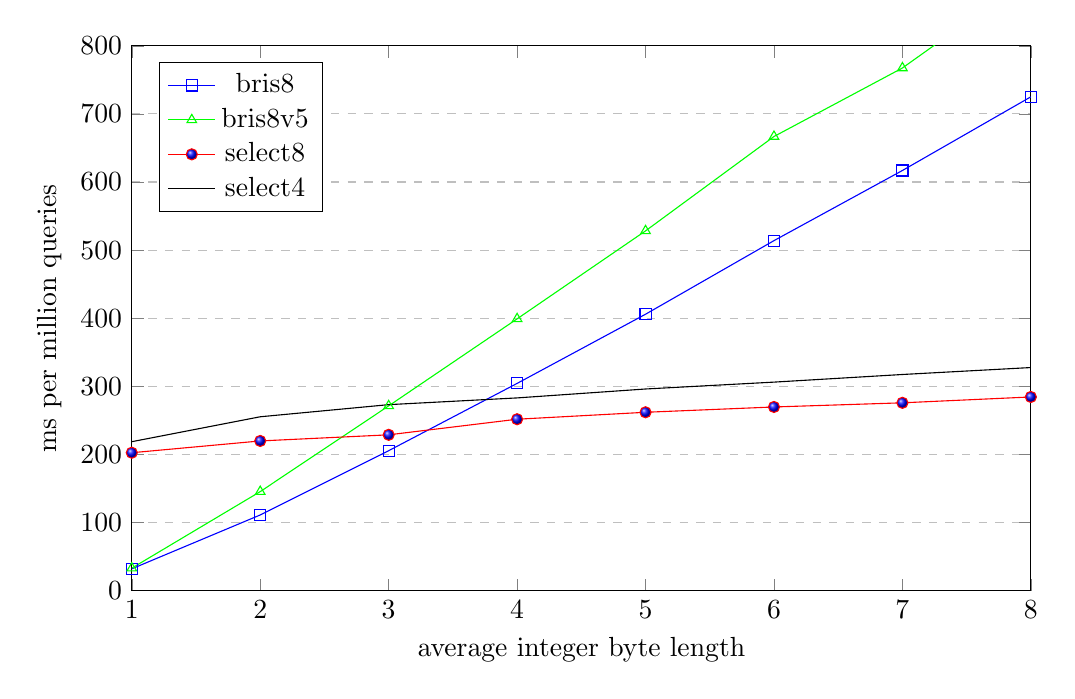
\begin{tikzpicture}
\begin{axis}[
    xlabel={average integer byte length},
    ylabel={ms per million queries},
    xmin=1, xmax=8,
    ymin=0, ymax=800,
    xtick={1,2,3,4,5,6,7,8},
    ytick={0,100,200,300,400,500,600,700,800},
    legend pos=north west,
    ymajorgrids=true,
    grid style=dashed,
    width=13cm, height=8.5cm
]

\addplot[
color=blue,
mark=square,
]
coordinates {
(1,31.90)(2,111.00)(3,205.40)(4,304.20)(5,405.80)(6,513.90)(7,616.90)(8,725.10)
};
\addplot[
color=green,
mark=triangle,
]
coordinates {
(1,32.90)(2,145.30)(3,271.20)(4,399.00)(5,528.20)(6,666.80)(7,767.40)(8,902.00)
};
\addplot[
color=red,
mark=ball,
]
coordinates {
(1,202.40)(2,219.70)(3,228.70)(4,251.60)(5,261.80)(6,269.60)(7,275.70)(8,284.30)
};
\addplot[
color=black,
mark=line,
]
coordinates {
(1,218.60)(2,255.20)(3,273.00)(4,282.90)(5,296.00)(6,306.10)(7,317.30)(8,327.50)
};

\legend{bris8, bris8v5, select8, select4 }


\end{axis}
\end{tikzpicture}
\caption{Rank and select performances} \label{graph:data_comparison}
\end{figure}

\section{Memory usage}
Tables~\ref{table:results8bit} and~\ref{table:results4bit} show memory size requirements for $rank$ and $select$ data structures with data sets consisting
 of 50 million 64-bit numbers. The compressed size column has a sum of continuation bit array and the data blocks. For $rank$ and $select$ methods used in this thesis, the total 
space taken by the extra data structures is only a small fraction of the overall size.

The static memory requirement of $select$ is easily noticeable, 
as is the relation between the memory requirement of $rank$ and the total number of blocks. Data structures in versions with smaller block size naturally take more space, but smaller block 
size allows better compression in some data sets and therefore a smaller total size. This can be seen when comparing the two forementioned figures: All 4-bit versions of the algorithms require
more space than the 8-bit versions, but the compressed size of the data is significantly smaller in the bottom two data sets. The data structure memory usage for the bottom row is similar in both versions 
due to the fact that the continuation bit array is exactly the same.




\begin{table}
\centering
\begin{tabular}{l|| c c c c } 
dataset   & compressed size & bris8  & bris8v5 & select8  \\
 \hline \hline 
all       & 168.4MB         & 4.67MB & 1.17MB   & 1.54MB    \\
twolarge  & 112.4MB         & 3.12MB & 781kB    & 1.48MB    \\
onelarge  &  63.2MB         & 1.76MB & 439kB    & 1.43MB    \\
onlysmall &  56.3MB         & 1.56MB & 391kB    & 1.43MB    \\


\hline
%
\end{tabular}
\caption{Memory requirement for 50M 64-bit numbers 8bit blocks, smaller is better.\label{table:results8bit}}
\end{table}

\begin{table}
\centering
\begin{tabular}{l|| c c c c } 
dataset   & compressed size & bris4  & bris4v5 & select4  \\
 \hline \hline 
all       & 177.7MB         & 7.65MB & 1.91MB  & 1.63MB \\
twolarge  & 116.1MB         & 4.66MB & 1.14MB  & 1.54MB \\
onelarge  & 42.5MB          & 2.12MB & 531kB   & 1.44MB \\
onlysmall & 31.3MB          & 1.56MB & 391kB   & 1.43MB \\


\hline
%
\end{tabular}
\caption{Memory requirement for 50M 64-bit numbers 4bit blocks, smaller is better.\label{table:results4bit}}
\end{table}

\section{Subarray access results}

The subarray access experiments were run similarly to the previous experiments. The data sets used contained 50 million numbers each. Most of the numbers were 4-bit long, with a varying amount of 32-bit 
integers randomly among them. The numbers in the x-axis correspond to the number of 32-bit integers per 1000 integers. One million indexes were randomized and both the index numbers and the data sets were 
preloaded into memory. A subarray of length 50 was decompressed from each randomized index location. Some precaution was used in the index randomizing to prevent reading from an out of bounds location.

Figure~\ref{graph:subarray} shows results for subarray fetching. The probability of having a long integer within the subarray range is visible from the results of the $rank$ based methods. When the density of the long integers increase, so does the need to access multiple 
block layers and thus the average time increases. The results of the $select$ based methods visualize the static need of singular $select$ query. The 4-bit version of $select$ requires a few more instructions 
during the block location phase and therefore is a little bit slower overall.


\begin{figure}[ht]
\centering
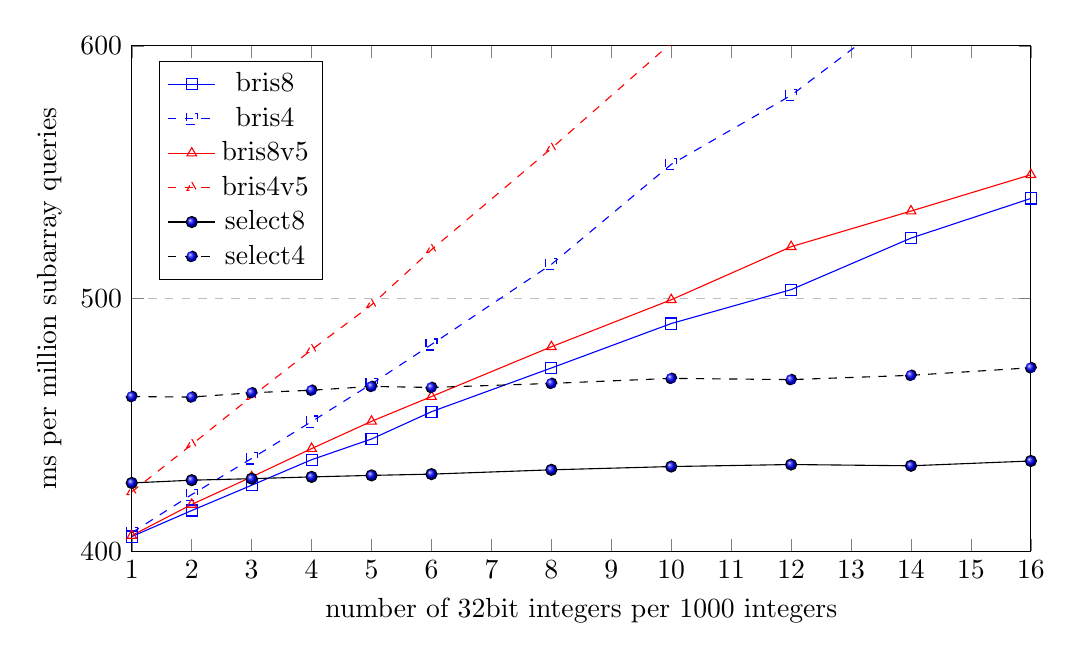
\begin{tikzpicture}
\begin{axis}[
    xlabel={number of 32bit integers per 1000 integers},
    ylabel={ms per million subarray queries},
    xmin=1, xmax=16,
    ymin=400, ymax=600,
    xtick={1,2,3,4,5,6,7,8,9,10,11,12,13,14,15,16},
    ytick={300,400,500,600,700},
    legend pos=north west,
    ymajorgrids=true,
    grid style=dashed,
    width=13cm, height=8cm
]

\addplot[
color=blue,
mark=square,
]
coordinates {
(1,405.80)(2,416.10)(3,426.10)(4,436.20)(5,444.40)(6,455.20)(8,472.50)(10,490.10)(12,503.50)(14,523.90)(16,539.60)(18,553.90)(20,564.80)(25,596.60)
};
\addplot[
color=blue, dashed,
mark=square,
]
coordinates {
(1,407.30)(2,422.40)(3,436.70)(4,451.30)(5,466.20)(6,481.80)(8,513.50)(10,553.10)(12,580.40)(14,616.30)(16,653.80)(18,685.80)(20,713.40)(25,810.70)
};
\addplot[
color=red,
mark=triangle,
]
coordinates {
(1,406.20)(2,418.50)(3,429.40)(4,440.60)(5,451.40)(6,461.20)(8,480.90)(10,499.50)(12,520.50)(14,534.60)(16,549.00)(18,570.10)(20,591.00)(25,625.20)
};
\addplot[
color=red, dashed,
mark=triangle, 
]
coordinates {
(1,423.50)(2,442.20)(3,461.20)(4,479.70)(5,497.50)(6,519.30)(8,559.40)(10,601.10)(12,642.60)(14,688.50)(16,728.40)(18,769.20)(20,793.00)(25,893.50)
};
\addplot[
color=black,
mark=ball,
]
coordinates {
(1,427.00)(2,428.10)(3,428.70)(4,429.40)(5,430.00)(6,430.50)(8,432.20)(10,433.50)(12,434.30)(14,433.80)(16,435.70)(18,436.90)(20,437.90)(25,440.80)
};
\addplot[
color=black, dashed,
mark=ball, 
]
coordinates {
(1,461.20)(2,461.00)(3,462.70)(4,463.70)(5,465.20)(6,464.80)(8,466.40)(10,468.40)(12,467.90)(14,469.60)(16,472.60)(18,472.70)(20,475.80)(25,480.60)
};


\legend{bris8, bris4, bris8v5, bris4v5, select8, select4 }

\end{axis}
\end{tikzpicture}
\caption{$Rank$ and $select$ performance with subarray fetching} \label{graph:subarray}
\end{figure}

\chapter{Conclusions and Future work}

When the dataset contains mostly small integers, the $rank$ based method by Brisaboa et al. is superior to the proposed $select$ based method. The benefit of using a direct array index instead of a $rank$ 
call for the first block gives a huge advantage. The $rank$ query is also slightly faster than a $select$ query, and therefore the dataset needs to have a large portion of longer elements. This can be seen 
from figure~\ref{graph:data_comparison}.

The order of how data is stored with $select$ compression enables an efficient fetching of a subarray. Only one $select$ query is needed in the beginning, and the decoding of the elements past the first one 
consists of just a few bit operations. 


There has already been a few successful attempts to decompress VB encoded integers with SIMD instructions \citep{Lem18,Pla15}. It is worthwhile to check if the select-based approach presented 
in this thesis benefits from SIMD. The data needs less manipulation because the data is already stored in the correct order, but calculating the integer block lengths might benefit from SIMD.

Another improvement to VB encoding is to see whether the compressed numbers can be changed. This is trivial until the block length of the compressed number changes. Then an additional data structure or 
cache is needed and the supporting rank/select data structure needs to be recalculated.

TODO:
 - see how cache matters

 - figure out why data size matters

 - more text / references

 - find ACL classifications
 
 - write keywords

 - remove lists from algorithms and data sets in results, explain whe data sets were roughly chosen like that

 - a real life situation where to use subarray


 - explain rank/select in introduction

 - 1.1 research questions



